% main.tex for multinotes/dev

% uncomment for handout version
\PassOptionsToPackage{blanks}{multinotes}
%\PassOptionsToPackage{noproofs}{multinotes}
%\PassOptionsToPackage{noanswers}{multinotes}
%\PassOptionsToPackage{blankproofs}{multinotes}
%\PassOptionsToPackage{blankanswers}{multinotes}
%\PassOptionsToPackage{student}{multinotes}
%\PassOptionsToPackage{slides}{multinotes}

%------------------------------------------------
\documentclass{article}
\usepackage[english,cleanlook]{isodate}
%------------------------------------------------

% paper
\usepackage[margin=30mm, a4paper]{geometry}
\setlength{\parindent}{0em}
\setlength{\parskip}{0.5em}

% multinotes
\usepackage{multinotes}

\textcolour{black}
\backgroundcolour{yellow!4}
\proofcolour{blue}
\answercolour{red}
\showcolour{purple}

\framedblankboxes
\framedproofs
\framedanswers
\setboxrule{0.5pt}

\setstretchfactor{1.2} 
\setimagestretchfactor{1}

\loadbabel

%% MOVE TO cerigos.sty (local styles)
%% meta info
%\institution{Cardiff University}
%\department{School of Mathematics}
%\modulecode{MAXXXX}
%\moduletitle{Test Module}
%\moduleterm{Autumn 2020}

% fonts
%\usepackage{stix}

% images
\usepackage{graphicx}
\usepackage{caption}
\usepackage{subfigure}
\graphicspath{{./figures/}}
\DeclareGraphicsExtensions{.png,.pdf,.jpeg,.jpg}


% theorems
% \theoremname, \lemmaname etc. are defined in multinotes.sty
\usepackage{amsthm}
\newtheoremstyle{break}{}{}{\upshape}{}{\bfseries}{\rule[-2ex]{0pt}{0pt}}{\newline}{}
\theoremstyle{break}
\newtheorem{theorem}{\theoremname}
\newtheorem{lemma}[theorem]{\lemmaname}
\newtheorem{proposition}[theorem]{\propositionname}
\newtheorem{corollary}[theorem]{\corollaryname}
\newtheorem{definition}[theorem]{\definitionname}
\newtheorem{remark}[theorem]{\remark}
\newtheorem{example}[theorem]{\examplename}
\newtheorem{exercise}[theorem]{\exercisename}
\newtheorem{quiz}[theorem]{\quizname}
\providecommand{\qed}{\par\mbox{}\hfill$\square$}

% hyperref
\usepackage[hidelinks]{hyperref}
\setcounter{tocdepth}{2}

% misc packages for testing
\usepackage{lipsum}
\usepackage{graphicx}
\usepackage{fancyvrb}

% language hacks
\let\oldsection=\section
\def\bsection#1#2{\oldsection{\ency{#1}{#2}}}
\let\oldsubsection=\subsection
\def\bsubsection#1#2{\oldsubsection{\ency{#1}{#2}}}

% teletype backslash for use in section titles 
\newcommand{\vbs}{\char`\\}

%% custom blank box
%\newenvironment{sketch}{
%	\begin{blankbox}[\sl Sketch]
%}{
%	\end{blankbox}
%}

% document info
\usepackage[english,cleanlook]{isodate}
\title{Typesetting lecture notes with {\tt multinotes.sty}}
\author{D Evans}

%\newcommand{\tmp}[1][]{}
%------------------------------------------------
\begin{document}
\maketitle
\bigskip\hrule\bigskip
\tableofcontents
%\listoffigures
%\listoftables
%\listof{video}{List of Videos}

\newpage

%------------------------------------------------
\section{Options}
%------------------------------------------------

The following package options are available.
\begin{table}[htb]
\renewcommand{\arraystretch}{1.3}
\addtolength{\tabcolsep}{2ex}
\begin{tabular}{lll}
\hline\hline
Option				& Effect \\
\hline\hline
{\tt blanks}		& \verb+\blank+ macros and \verb+blankbox+ environments replaced by whitespace \\
{\tt noproofs}		& proofs excluded \\
{\tt blankproofs}	& proofs replaced by whitespace \\
{\tt noanswers}		& answers excluded \\
{\tt blankanswers}	& answers replaced by whitespace \\
\hline
{\tt langA}			& include {\tt langA} content \\
{\tt langA, langB}	& include {\tt langA} and {\tt langB} content \\
\hline
{\tt parallel}		& typeset languages simultaneously in separate columns \\
{\tt slides}		& landscape mode with screen fonts \\
\hline\hline
\end{tabular}
\end{table}

%----------------------------------------
\subsection{Preamble commands}
%----------------------------------------

\framebreak
The following preamble commands are available.
\begin{table}[htb]
\renewcommand{\arraystretch}{1.3}
\addtolength{\tabcolsep}{2ex}
\begin{tabular}{lll}
\hline\hline
Command							& \hspace{0.3\textwidth}\mbox{}\\
\hline\hline
\verb+\textcolour{}+			&  set text colour\\
\verb+\backgroundcolour{}+		&  set background colour \\
\verb+\showcolour{}+			&  set text colour of blank boxes\\
\verb+\proofcolour{}+			&  set text colour of proofs \\
\verb+\answercolour{}+			&  set text colour of answer boxes \\
\hline
\verb+\framedblankboxes+		&  for framed blankboxes \\
\verb+\framedproofs+			&  for framed proofs\\
\verb+\framedanswers+			&  for framed anwers\\
\verb+\setboxrule{}+			&  set frame thickness\\
\hline
\verb+\setstretchfactor{}+		&  to accomodate handwriting in blank boxes\\
\verb+\setimagestretchfactor{}+	&  to accomodate hand-drawing in blank boxes\\
\hline\hline
\end{tabular}
\end{table}

%------------------------------------------------
\section{Inline boxes}
%------------------------------------------------
The following macros replace their content by whitespace in response to differnet options. These can be used for partial handouts to accompany lectures or videos, or for missing-word exercises etc.
\begin{itemize}
\item \verb+\blank{...}+ is emptied by the {\tt blanks} option.
\item \verb+\fillbox{...}+ is emptied by {\tt blankanswers} and {\tt noanswers}.
\item \verb+\ans{...}+ is emptied by {\tt blankanswers} and removed for {\tt noanswers}.
\end{itemize}

%----------------------------------------
\subsection{\tt\vbs blank}
%----------------------------------------
Inline text is replaced by whitespace.

\begin{Verbatim}[frame=single]
Here is some \blank{text} to be hidden.
\end{Verbatim}
Here is some \blank{text} to be hidden.


%----------------------------------------
\subsection{\tt\vbs fillbox}
%----------------------------------------
Similar to \verb+\blank+ but controlled by the \verb+blankanswers+ option.

\begin{Verbatim}[frame=single]
Roses are \fillbox{red}, violets are \fillbox{blue}.
\end{Verbatim}
Roses are \fillbox{red}, violets are \fillbox{blue}.

%----------------------------------------
\subsection{\tt\vbs ans}
%----------------------------------------
Similar to \verb+\fillbox+ but also controlled by the \verb+noanswers+ option.
\begin{itemize}
\item {\tt blankanswers} replaces the content by blank space. 
\item {\tt noanswers} removes the answer completely.
\end{itemize}

\begin{Verbatim}[frame=single]
What is $7\times 8$? \ans{54}
\end{Verbatim}
What is $7\times 8$\,? \ans{54}

%\begin{exercise}
%\mbox{}\vspace*{-2\baselineskip}
%\begin{questions}
%\question\quad Roses are \blank{red}, violets are \blank{blue}.
%\question\quad $\blank{3} + 4 = 7$
%\question\quad $5 - \blank{2} = 3$
%\end{questions}
%\end{exercise}
%
%TODO Answers need to be shown inside the boxes!

%------------------------------------------------
\section{Display boxes}
%------------------------------------------------
The following environments replace displayed content by whitespace. The \verb+proof+ and \verb+answer+ environments can also be removed entirely (courtesy of the \verb+comment+ package).
\begin{itemize}
\item \verb+\begin{blankbox}...\end{blankbox}+ is controlled by the \verb+blank+ option.
\item \verb+\begin{proof}...\end{proof}+ is controlled by \verb+blankproofs+ and \verb+noproofs+.
\item \verb+\begin{answer}...\end{answer}+ is controlled by \verb+blankanswers+ and \verb+noanswers+.
\end{itemize}

%----------------------------------------
\subsection{The {\tt blankbox} environment}
%----------------------------------------

\subsubsection{A simple {\tt blankbox}}

\begin{Verbatim}[frame=single]
\begin{blankbox}
\lipsum[1]
\end{blankbox}
\end{Verbatim}
\begin{blankbox}
\lipsum[1]
\end{blankbox}

\subsubsection{A {\tt blankbox} with an optional title}

\begin{Verbatim}[frame=single]
\begin{blankbox}[\sl Some ideas]
\lipsum[13]
\end{blankbox}
\end{Verbatim}
\begin{blankbox}[\sl Some ideas]
\lipsum[13]
\end{blankbox}

%\subsubsection{A {\tt blankbox} inside a theorem-like environment}
%
%\begin{example}
%What is $P(X\leq 2)$ when $X\sim\text{Poisson}(\lambda)$?
%\begin{blankbox}[\sl Solution]
%\[
%P(X=k) = \displaystyle\frac{\lambda^ke^{-\lambda}}{k!}
%\quad\text{so}\quad
%P(X\leq 2) = \left(1 + \lambda + \frac{\lambda^2}{2}\right)e^{-\lambda}.
%\]
%\end{blankbox}
%\end{example}
%\begin{Verbatim}[frame=single]
%\begin{example}
%What is $P(X\leq 2)$ when $X\sim\text{Poisson}(\lambda)$?
%\begin{blankbox}[\sl Solution]
%\[
%P(X=k) = \displaystyle\frac{\lambda^ke^{-\lambda}}{k!}
%\quad\text{so}\quad
%P(X\leq 2) = \left(1 + \lambda + \frac{\lambda^2}{2}\right)e^{-\lambda}.
%\]
%\end{blankbox}
%\end{example}
%\end{Verbatim}

\subsubsection{A custom {\tt blankbox} environment}
Custom boxes controlled by the {\tt blank} option can be defined as follows.
%
\begin{Verbatim}[frame=single]
\newenvironment{solution}{
    \begin{blankbox}[\sl Sol.]
}{
    \end{blankbox}
}
\begin{solution}
Blah, blah ...
\end{solution}
\end{Verbatim}

\newenvironment{solution}{
	\begin{blankbox}[\sl Sol.]
}{
	\end{blankbox}
}
\begin{solution}
Blah, blah ...
\end{solution}

%\begin{Verbatim}[frame=single]
%\renewcommand{\notesname}{\bf Nodiadau}
%\begin{notes}
%...
%\end{notes}
%\end{Verbatim}
%\renewcommand{\notesname}{\bf Nodiadau}
%\begin{notes}
%\lipsum[4]
%\end{notes}

%----------------------------------------
\subsection{The {\tt proof} environment}
%----------------------------------------
\begin{itemize}
\item {\tt blankproofs} replaces the contents by blank space. 
\item {\tt noproofs} removes the proof completely.
\end{itemize}

The {\tt noproofs} option is implemented using the {\tt comment} package. For it to work properly, the opening and closing commands \verb+\begin{proof}+ and \verb+\end{proof}+ must each appear on a line of its own, with no additional whitespace. This also applies to the \verb+answer+ environment and {\tt noanswers} option (see below).

Here is a proof (might be removed).
\begin{proof}
\lipsum[13]
\qed
\end{proof}

This is produced by the following code.
\begin{Verbatim}[frame=single]
\begin{proof}
...
\end{proof}
\end{Verbatim}

% change proof title
Here is a proof with a custom title (might be removed).
\begin{proof}[\sl Proof of main theorem]
\lipsum[13]
\qed
\end{proof}

This is produced by the following code.
\begin{Verbatim}[frame=single]
\begin{proof}[\sl Proof of main theorem]
...
\end{proof}
\end{Verbatim}

%----------------------------------------
\subsection{The {\tt answer} environment}
%----------------------------------------

\begin{itemize}
\item {\tt blankanswers} replaces the content by blank space. 
\item {\tt noanswers} removes the answer completely.
\end{itemize}

Here is an answer environment (might be removed).
\begin{answer}
\lipsum[1]
\end{answer}

This is produced by the following code.
\begin{Verbatim}[frame=single]
\begin{answer}
...
\end{answer}
\end{Verbatim}

Here is an answer environment with a custom title (might be removed)

\renewcommand{\answername}{\bf Ans.}
\begin{answer}
\lipsum[1]
\end{answer}

This is produced by the following code.
\begin{Verbatim}[frame=single]
\renewcommand{\answername}{\bf Ans.}
\begin{answer}
...
\end{answer}
\end{Verbatim}

%----------------------------------------
\section{Questions, choices and checkboxes}
%------------------------------------------------

The package replicates the list environments found in {\tt exam.cls}, namely {\tt questions}, {\tt parts}, {\tt subparts}, {\tt choices} and {\tt checkboxes} and makes them responsive to {\tt blankanswers} and {\tt noanswers}. For example,

\begin{Verbatim}[frame=single]
\begin{exercise}\label{exe:demo}
\begin{questions}
\question What is $7\times 8$? \ans{54}
\question State Pythagoras' theorem. \ans{$a^2+b^2=c^2$}
\end{questions}
\end{exercise}
\end{Verbatim}

%Here is a list of questions inside a (theorem-like) exercise environment.
%\begin{exercise}
%\begin{questions}
%\item[] % for a linebreak
%\question A
%\begin{parts}
%\part AA
%\begin{subparts}
%\subpart  AAA
%\subpart AAB
%\end{subparts}
%\part AB
%\begin{subparts}
%\subpart  ABA
%\subpart ABB
%\end{subparts}
%\end{parts}
%\question B
%\begin{parts}
%\part BA
%\begin{subparts}
%\subpart  BAA
%\subpart BAB
%\end{subparts}
%\part BB
%\begin{subparts}
%\subpart  BBA
%\subpart BBB
%\end{subparts}
%\end{parts}
%\end{questions}
%\end{exercise}

% exercise
\bigskip
Here is a list of questions inside a (theorem-like) exercise environment.
\begin{exercise}\label{exe:demo}
\begin{questions}
\item[] % for a linebreak
\question First question.
\begin{parts}
\part First part \ans{Answer to first part.}
\part Second part
\begin{subparts}
\subpart First subpart. \ans{Answer to first subpart.}
\subpart Second subpart. \ans{Answer to second subpart.}
\end{subparts}
\part Third part \ans{Answer to third part.}
\end{parts}
\question Second question \ans{Answer to second question.}
\end{questions}
\end{exercise}
%
%--------------------
\subsection{Multiple choice questions}

In what year did Columbus first cross the Atlantic?
\begin{choices}
\choice 1490 
\choice 1491 
\correctchoice 1492 
\choice 1493 
\end{choices}

This is produced by the following code.
\begin{Verbatim}[frame=single]
In what year did Columbus first cross the Atlantic?
\begin{choices}
\choice 1490 
\choice 1491 
\correctchoice   1492 
\choice 1493 
\end{choices}
\end{Verbatim}

\subsection{Multiple answer questions}

Which of the following were members of the Beatles?
\begin{checkboxes}
\correctchoice John
\correctchoice Paul
\correctchoice George
\choice Zippy
\end{checkboxes}

This is produced by the following code.
\begin{Verbatim}[frame=single]
Which of the following were members of the Beatles?
\begin{checkboxes}
\correctchoice John
\correctchoice Paul
\correctchoice George
\choice Zippy
\end{checkboxes}
\end{Verbatim}

\bigskip
\begin{quiz}
Here is a (theorem-like) quiz with a fill-the-blanks question, a true-or-false question, a multiple choice question, and a multiple answer question.

\begin{Verbatim}[frame=single]
Roses are \fillbox{red}, violets are \fillbox{blue}.
\end{Verbatim}

\begin{questions}
% FIL
\question
Fill in the blanks: {\sl
	Roses are \fillbox{red}, violets are \fillbox{blue}.
}


% TF question
\question\label{qu:rain}
The rain in Spain falls mainly on the plain.
\begin{choices}
\correctchoice True 		
\choice False		
\end{choices}

% MC question
\question\label{qu:america}
In what year did Columbus first cross the Atlantic?
\begin{choices}
\choice 1490 
\choice 1491 
\correctchoice 1492
\choice 1493 
\end{choices}

% MA question 
\question\label{qu:beatles}
Which of the following were members of the Beatles?
\begin{checkboxes}
\correctchoice John
\correctchoice Paul
\correctchoice George
\choice Bingo
\end{checkboxes}

\end{questions}
\end{quiz}

%------------------------------------------------
\section{Videos}
%------------------------------------------------
For PDF output, video content is rendered as hyperlinks.

%----------------------------------------
\subsection{\tt\vbs includevideo}
%----------------------------------------
The \verb+\includevideo+ command mirrors \verb+\includegraphics+. 

\begin{Verbatim}[frame=single]
\includevideo[scale=0.5]{https://www.youtube.com/embed/oCDXhvXye9E}
\end{Verbatim}

%----------------------------------------
\subsection{The {\tt video} environment}
%----------------------------------------

A new float called {\tt video} mimics the {\tt figure} and {\tt table} environments. These can be framed and captioned. A corresponding \verb+\listofvideos+ (suffix {\tt .lov}) can be included.

\begin{Verbatim}[frame=single]
\begin{video}
\centering
\includevideo[scale=0.5]{https://www.youtube.com/embed/oCDXhvXye9E}
\caption{Proof of theorem~1\label{vid:pf1}}
\end{video}
\end{Verbatim}

\begin{video}
\centering
\includevideo{https://www.youtube.com/embed/oCDXhvXye9E}
\caption{Proof of theorem~1\label{vid:pf1}}
\end{video}

%\begin{video}
%\centering
%\includevideo[scale=0.5]{https://www.youtube.com/embed/d22CiKMPpaY}
%\caption{As time goes by\label{vid:as-time-goes-by}}
%\end{video}
%
%\begin{video}
%\centering
%\includevideo[scale=0.5]{https://www.youtube.com/embed/wqGUwL0P6no}
%\caption{Optimistic voices\label{vid:optimistic-voices}}
%\end{video}


%------------------------------------------------
\section{Images}
%------------------------------------------------

%----------------------------------------
\subsection{\tt\vbs includegraphics}
%----------------------------------------
\verb+\includegraphics{img}+ replaces \verb+img+ by whitespace whenever the {\tt blanks} option is set.


\begin{Verbatim}[frame=single]
\begin{blankbox}
\resizebox{0.3\textwidth}{!}{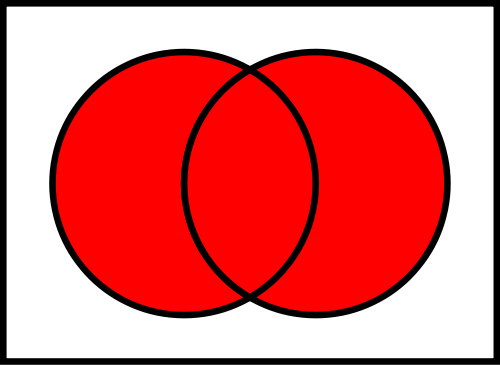
\includegraphics{AcupB}}
\end{blankbox}
\end{Verbatim}

\begin{blankbox}
\resizebox{0.3\textwidth}{!}{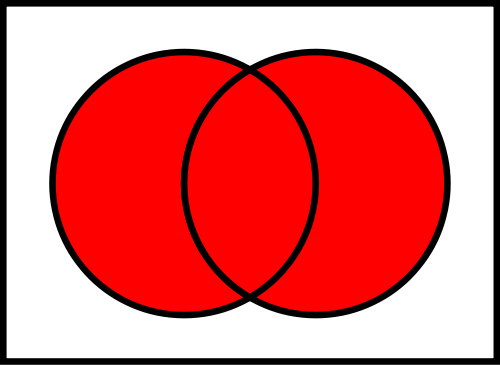
\includegraphics{AcupB}}
\end{blankbox}

%----------------------------------------
\subsection{\tt\vbs includetwographics}
%----------------------------------------

\verb+\includetwographics{img1}{img2}+ shows \verb+img2+ whenever {\tt blanks}, {\tt blankproofs} or {\tt blankanswers} is set, otherwise it shows \verb+img1+. This can be used to print partial images in handout notes and exercise sheets. 

\begin{Verbatim}[frame=single]
\begin{blankbox}
\resizebox{0.3\textwidth}{!}{\includetwographics[scale=1]{AcupB}{emptyset}}
\resizebox{0.3\textwidth}{!}{\includetwographics[scale=1]{AcapB}{emptyset}}
\resizebox{0.3\textwidth}{!}{\includetwographics[scale=1]{Acomp}{emptyset}}
\end{blankbox}
\end{Verbatim}

\begin{blankbox}
\resizebox{0.3\textwidth}{!}{\includetwographics[scale=1]{AcupB}{emptyset}}
\resizebox{0.3\textwidth}{!}{\includetwographics[scale=1]{AcapB}{emptyset}}
\resizebox{0.3\textwidth}{!}{\includetwographics[scale=1]{Acomp}{emptyset}}
\end{blankbox}


%----------------------------------------
\subsection{TikZ}
%----------------------------------------

% create random walk picture
\usetikzlibrary{math}
\usetikzlibrary{calc}
\tikzset{every picture/.style={line width=1pt}}
\tikzset{every picture/.append style={x=1cm,y=0.5cm}}
\tikzset{every picture/.append style={font=\Large}}
\pgfmathsetseed{\number\pdfrandomseed}
\tikzset{
	axes/.pic={
	\draw[help lines, color=gray!30, dashed] (-0.9,-9.9) grid (10.9,9.9);
	\draw[->,thick] (-1,0)--(11,0) node[right]{$t$};
	\draw[->,thick] (0,-10)--(0,10) node[above]{$x$};
	}
}
\tikzset{
	samplepaths/.pic={
		\foreach \c in {red, green, blue}
		    \draw [\c] (0,0) \foreach ~ in {0,...,10}{-- ++(1,{random(0,1)*2-1})};
	}
}
\tikzset{
    rwalk/.pic={
        \pic{axes};
        \pic{samplepaths};
    }
}

% tikz picture
%\begin{Verbatim}[frame=single]
%\resizebox{0.5\textwidth}{!}{\tikz\pic{rwalk};}
%\end{Verbatim}
%
%\begin{figure}[htb]
%\centering
%\resizebox{0.5\textwidth}{!}{\tikz\pic{rwalk};}
%\caption{A random walk!\label{fig:rwalk}}
%\end{figure}


% show 
Here is a tikz pcture in a blankbox. The \verb+\blanktikz+ command should make it disappear when the {\tt blanks} option is set.
\begin{Verbatim}[frame=single]
\begin{blankbox}
\blanktikz
\resizebox{0.5\textwidth}{!}{\tikz\pic{rwalk};}
\end{blankbox}
\end{Verbatim}

\showcolour{black}
\begin{blankbox}
\blanktikz
\resizebox{0.5\textwidth}{!}{\tikz\pic{rwalk};}
\end{blankbox}
%

%------------------------------------------------
\section{Slides}
%------------------------------------------------

The \verb+slides+ option produces a landscape document with big fonts. The package defines the macro \verb+\framebreak+. This produces a \verb+\newpage+ when the \verb+slides+ option is set, but otherwise has no effect. There is some scope to extend this functionality. Landscape mode is handy for bilingual (two-column) documents.


%------------------------------------------------
\appendix
%------------------------------------------------

%------------------------------------------------
\newpage
\section{Prime numbers quiz}
%------------------------------------------------

\begin{questions}

\question
What are the prime factors of 42?
\begin{choices}
\choice $3\times 14$
\correctchoice $2\times 3\times 7$
\choice $2\times 21$
\end{choices}

\question
What are the prime factors of 150?
\begin{choices}
\correctchoice $2\times 3\times 5\times 5$
\choice $3\times 3\times 5\times 5$
\choice $6\times 25$
\end{choices}

\question
What is the LCM of 13 and 3?
\begin{choices}
\choice $13$
\choice $3$
\correctchoice $39$
\end{choices}

\question
What is the HCF of 32 and 24?
\begin{choices}
\choice $2$
\correctchoice $8$
\choice $4$
\end{choices}

\question
What is the LCM of 24 and 36?
\begin{choices}
\choice $12$
\correctchoice $72$
\choice $30$
\end{choices}

\question
What is the HCF of 104 and 136?
\begin{choices}
\correctchoice $8$
\choice $12$
\choice $13$
\end{choices}

\question
What is the HCF of $3\times 13$ and $2^2\times 13$?
\begin{choices}
\choice $9$
\choice $17$
\correctchoice $13$
\end{choices}

\newpage % << remove
\question
What is the LCM of $2^2\times 3^2\times 5$ and $2^3\times 3\times 5$?
\begin{choices}
\correctchoice $360$
\choice $16\,120$
\choice $30$
\end{choices}

\question
What is the HCF of $2\times 5\times 13$ and $22\times 13$?
\begin{choices}
\choice $13$
\correctchoice $26$
\choice $52$
\end{choices}

\question
Find the LCM of $3^2\times 11\times 13$ and $3\times 11^2$.
\begin{choices}
\choice $1287$
\correctchoice $14\,157$
\choice $429$
\end{choices}

\end{questions}


%------------------------------------------------
\end{document}
%------------------------------------------------


